%%=============================================================================
%% Methodologie
%%=============================================================================

\chapter{Methodologie van het Experiment}
\label{ch:methodologie}

Om de kwaliteit van een augmented reality framework te beoordelen is het experiment in twee delen opgedeeld. Het eerste deel van het experiment gaat over hoe goed de frameworks de core van de applicatie kunnen implementeren. Elk framework krijgt dezelfde lijst met vijftien verschillende afbeeldingen. De bedoeling is dat elk framework zoveel mogelijk images probeert te herkennen. De gebruikte lijst met images kan u vinden in de bijlage. De lijst is opgebouwd uit afbeeldingen met een verschillende moeilijkheidsgraad. Om te weten wat een moeilijke of makkelijke afbeelding is gebruikt deze studie volgende criteria.

\begin{itemize}
    \item Veel features
    \item Geen repetitieve features
    \item Goed contrast
\end{itemize} 


Het tweede deel van het experiment gaat over de performance van elk framework. Dit wordt gedaan door FPS, gereserveerd RAM en gealloceerd RAM met elkaar te vergelijken. Omdat ieder framework gebruik maakt van andere API's moet voor elk van deze een soortgelijke applicatie worden voorzien. Deze applicatie moet een afbeelding herkennen aan hierop een 3d object tonen. Bij het klikken op dit object verandert de kleur van rood naar blauw en omgekeerd. Het is de bedoeling dat bij het verliezen van de tracking van de afbeelding, en hierna terug tracken, het object nog steeds dezelfde kleur heeft.

\section{Profiling in Unity}
Met Unity zijn er verschillende mogelijkheden om een applicatie te monitoren. Unity zelf biedt een profiling tool aan die live toont hoeveel CPU, RAM, GPU... de applicatie gebruikt (zie figuur \ref{fig:unityprofiling}). Ook geeft deze tool voor elke meeteenheid nog extra informatie, bijvoorbeeld bij CPU Usage geeft de tool aan hoelang de functies duren. Het nadeel van deze tool is dat hij alleen maar de data kan tonen van de laatste honderdtal frames en deze niet kan exporteren naar een bestandsformaat dat compatibel is met een dataverwerkingsprogramma zoals Excel of R \autocite{UnityProfiling}.

\begin{figure}
    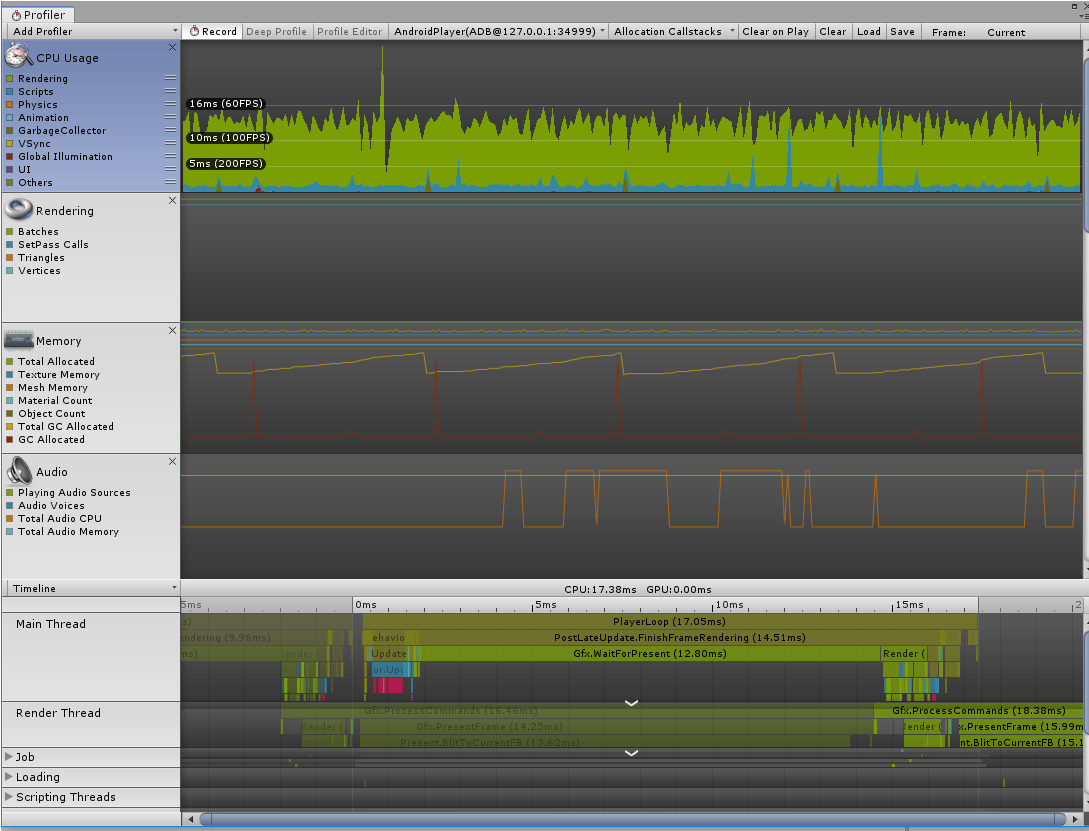
\includegraphics[width=\linewidth]{unityProfiling.png}
    \caption{Unity Profiling Tool}
    \label{fig:unityprofiling}
\end{figure}

Voor deze reden is er een zelfgemaakt script ontworpen om de nodige waarden weg te schrijven naar een csv bestand. Dit script berekent elke second de FPS door het totaal aantal frames van deze second te verminderen met het totaal aantal van de vorige second. Het gereserveerde en alloceerde RAM vraagt het script op aan de UnityEngine.Profiling.Profiler klasse die beide waarden bezit als variabelen. Het script schrijft ook het aantal gameObjects van Unity weg naar de csv, deze waarde kan aantonen wat er juist gebeurt met images eens ze hun tracking verliezen (zie script \ref{code:profilerScript}).

Het script is vast gemaakt aan een leeg gameObject (zonder andere scripts en componenten) om dit te kunnen laten runnen. Het script runt eenmalig zijn Start() functie wanneer het object is geïnitialiseerd en voert dan elke seconde berekening uit.

\codefragment{code/ExperimentProfiler.cs}{Custom Profiler Script}{code:profilerScript}

\section{Gebruikte Unity Componenten}
Omdat beide applicaties gebruik maken van Unity delen deze enkele componenten. Om duidelijk te maken wat deze doen volgt in deze sectie een uitleg van elk van deze componenten. Ook de profiler valt onder één van deze componenten.

\subsection{Scene}
Een scene bevat alle virtuele objecten en  UI elementen die tegelijk op het scherm aanwezig moeten zijn. Dit betekent echter niet dat het nodig is dat deze allemaal tegelijk actief zijn, deze objecten kunnen ook niet actief zijn waardoor ze wel aanwezig zijn (geheugen gebruik) maar niet op de scene zichtbaar zijn. Een applicatie kan bestaan uit meerdere scenes waardoor het mogelijk is om functionaliteiten op te splitsen in verschillende scenes. De scenes kunnen ook met elkaar communiceren om zo van de ene scene naar de andere over te gaan.

\subsection{Game object}
De standaard manier om een virtueel object te tonen is aan de hand van een gameobject. Dit gameobject bestaat uit verschillende componenten die bepalen hoe het object eruitziet. Deze kan ook nog scripts bevatten die de mogelijkheid bieden om verschillende acties uit te voeren wanneer een lifecycle methode voorkomt van een gameobject. Er zijn verschillende lifecycle methodes beschikbaar maar de meest gebruikte zijn Start (creatie object) en Update (elke frame).

Een gameobject moet niet altijd een fysieke vorm hebben, een leeg gameobject kan ook bestaan. Dit object kan dan nog steeds gebruikmaken van de lifecycle methoden. De profiler is hier een voorbeeld van.

\subsection{Canvas}
Het canvas bevat alle UI elementen zoals text, images en buttons.

\subsection{Camera}
De camera bepaalt welke delen van de scene getoond worden. Om de performance van applicaties met een groot aantal objecten te verbeteren maakt Unity gebruik van Occlusion en Frustum Culling om alleen objecten te tonen die zich in het gezichtsveld van de camera bevinden \autocite{UnityCulling}.

\subsection{Cube Touch}
Om geen grote externe invloed te hebben op beide applicaties delen deze hetzelfde virtuele object dat de applicatie toont bij de herkenning van de afbeelding. Dit object bevat een custom script dat detecteert wanneer de gebruiker op de kubus duwt via het smartphone scherm en zal deze van kleur veranderen.

\section{Applicatie ARCore}

\subsection{Image Database}
De ARCore database is aangemaakt door alle benodigde afbeeldingen toe te voegen aan de applicatie en deze te bundelen in een asset file. Deze file geeft aan elke afbeelding een score van 0 tot 100 (zie figuur \ref{fig:arcoreDatabase}). \textcite{GoogleImages} adviseert om alleen images te gebruiken met een score van minstens 75.

\begin{figure}
    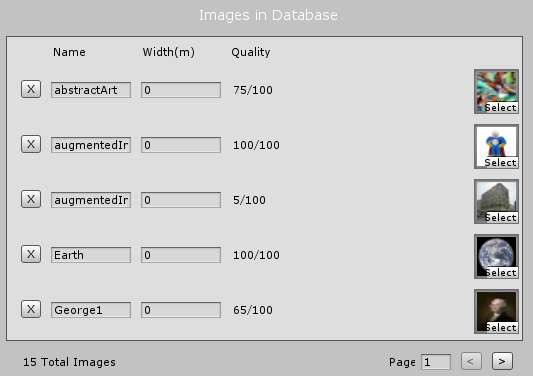
\includegraphics[width=\linewidth]{arcoreDatabase.png}
    \caption{ARCore database inclusief score}
    \label{fig:arcoreDatabase}
\end{figure}

In tegenstelling tot Vuforia heeft ARCore de mogelijkheid om tijdens runtime afbeeldingen toe te voegen aan deze databank.

\subsection{Configuratie}
ARCore maakt gebruik van een speciaal object genaamd 'ARCore Device' dat inbegrepen is bij de package van ARCore. Dit object bevat een script die als variabele een Session Config vraagt. Deze studie heeft gebruik gemaakt van de standaardconfiguratie die inbegrepen is. Bij deze configuratie was het alleen nog nodig om de aangemaakte database te selecteren.
Omdat de Session Config een variabele is, is het ook mogelijk om per scene een ander configuratiebestand te selecteren.

\subsection{Tracking via Controller Klasse}
Om afbeeldingen te herkennen is er een leeg gameobject nodig met een tracking script. Dit script zoekt via zijn update lifecycle methode welke afbeeldingen momenteel zichtbaar zijn. Wanneer een afbeelding zichtbaar is plaatst deze methode een ankerpunt en voegt hieraan het benodigde gameobject toe. Omdat deze applicatie voor elke image het dezelfde gameobject gebruikt creëert hij dit object op basis van de meegegeven prefab. Dit nieuw object bevat zelf ook een script dat instaat voor het beheren van zijn status wanneer de tracking verdwijnt (maar nog niet gestopt). Indien dit gebeurt zal deze zich op non-actief zetten waardoor hij niet meer zichtbaar is in de scene. Echter betekent dit niet dat de tracking gestopt is, wanneer de camera de image binnen een bepaalde tijd terug in zijn gezichtsveld heeft wordt deze terug actief. Dit zorgt ervoor dat de ervaring voor de gebruiker beter is omdat het object niet terug moet verschijnen wanneer deze eventjes wegkijkt van de afbeelding.

\section{Applicatie Vuforia}

\subsection{Image Database}
De Vuforia image database is aangemaakt via hun developer site. Hierop zijn de 15 afbeeldingen toegevoegd en hebben ze ook elk een score gekregen van 0 tot 5 sterren die aangeeft hoe makkelijk Vuforia de afbeelding kan herkennen (zie figuur \ref{fig:vuforiaDatabase}). Ook is er de mogelijkheid om per afbeelding de features te tonen die Vuforia gebruikt om een afbeelding te herkennen.

\begin{figure}
    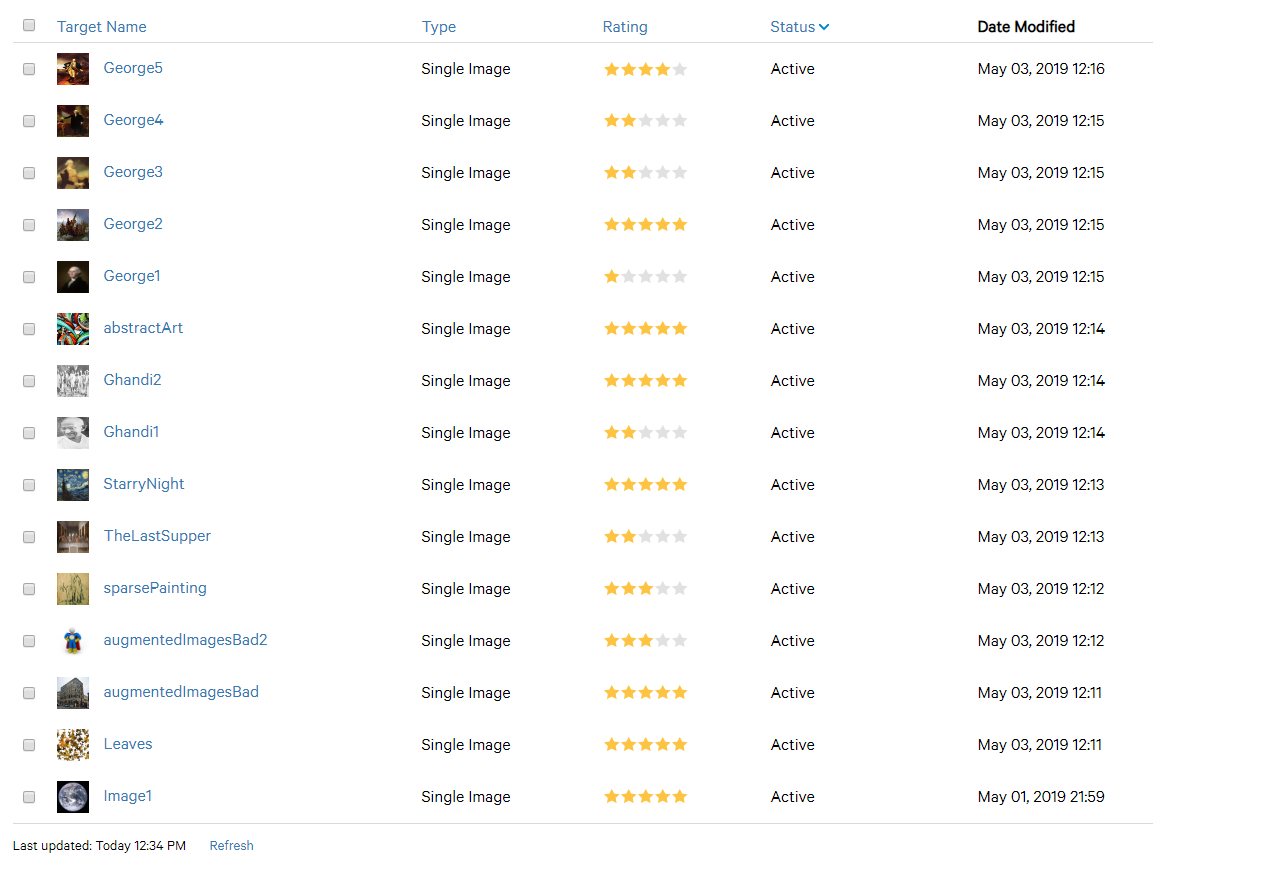
\includegraphics[width=\linewidth]{vuforiaSite.png}
    \caption{Lijst met de 15 images en hun score}
    \label{fig:vuforiaDatabase}
\end{figure}

\subsection{Configuratie}
Om ervoor te zorgen dat Vuforia optimaal gebruik maakt van de platform enablers (in dit geval ARCore) moet eerst de ARCore Unity SDK zich bevinden in het mapje `Assets/Android/Plugins', alleen dan zal Vuforia volledig gebruiken maken van de onderliggende ARCore SDK \autocite{VuforiaARCore}.

Het is ook heel belangrijk dat in de VuforiaConfiguration file bij 'Device Tracker' de optie 'Track Device Pose' is ingeschakeld. Deze optie zorgt ervoor dat Vuforia de image nog eventjes trackt wanneer deze fysiek niet meer zichtbaar is. Ook is hier de optie om te kiezen tussen een 'Positional' of 'Rotational' tracking mode, deze bepaalt het aantal beschikbare \acrlong{dof}. Omdat bij deze applicatie 'Track Device Pose' belangrijk is moet er positional tracking (\acrshort{6dof}) beschikbaar zijn.

\subsection{Tracking via Image Targets}
In tegenstelling tot ARCore maakt Vuforia niet gebruik van één enkele klasse om alle tracking te regelen. Per afbeelding die de applicatie moet herkennen is er een 'Image Target' object nodig. Dit object bestaat uit de standaard Unity elementen net zoals bij ARCore maar bevat ook enkele scripts die nodig zijn voor Vuforia. Het eerste script dat nodig is, is het 'Image Target behaviour' script. Dit script bepaalt welke database de image moet gebruiken en welke afbeelding hij moet herkennen. Een 'Turn off behaviour' script dat ervoor zorgt dat de afbeelding zelf niet wordt getoond wanneer de gebruiker de applicatie gebruikt en ook een 'Tracking' script dat ervoor zorgt dat het virtuele object verschijnt wanneer de afbeelding herkent wordt (zie figuur \ref{fig:vuforiaImageTarget}). 

Er is de mogelijkheid om voor al van deze scripts een eigen script te schrijven. Voor deze studie was het alleen nodig om een eigen 'Tracking' script te schrijven zodat de naam van de image op het scherm verschijnt. De overige functies erft dit script over van het standaard 'DefaultTrackingBehaviour' script.

\begin{figure}
    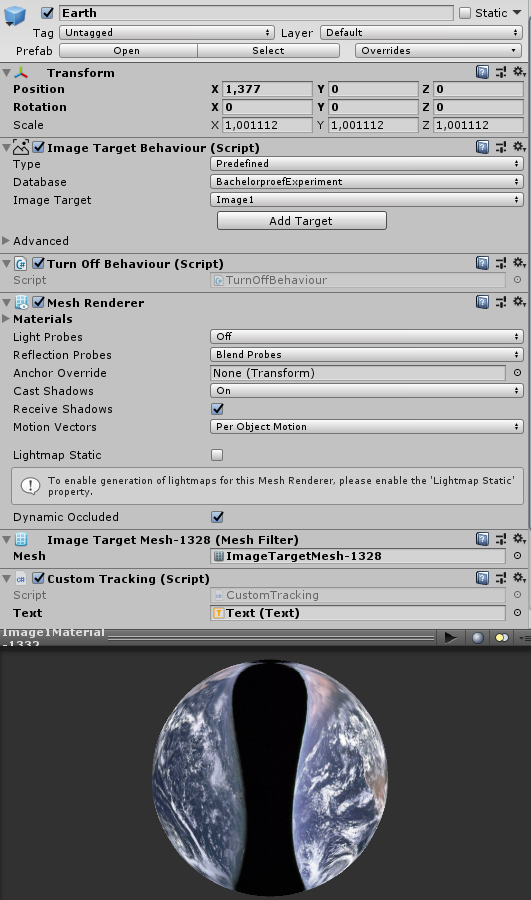
\includegraphics[width=\linewidth]{vuforiaImageTarget.png}
    \caption{Voorbeeld van een Image Target Object}
    \label{fig:vuforiaImageTarget}
\end{figure}

Om een virtueel object te binden aan de Image Target zijn er verschillende mogelijkheden. De standaard optie die Vuforia zelf aanraad op zijn site is om het object een kind te maken van het target. Op deze manier zal het DefaultTrackingBehaviour script, of scripts die hiervan overerven, de render-, collider- en canvas componenten van het object activeren bij de start van de tracking of deactiveren wanneer de tracking verloren gaat.

%% TODO: Hoe ben je te werk gegaan? Verdeel je onderzoek in grote fasen, en
%% licht in elke fase toe welke stappen je gevolgd hebt. Verantwoord waarom je
%% op deze manier te werk gegaan bent. Je moet kunnen aantonen dat je de best
%% mogelijke manier toegepast hebt om een antwoord te vinden op de
%% onderzoeksvraag.
